\documentclass[
    aps,
    prb, 
    twocolumn, superscriptaddress,
    amsmath,
    amssymb,
    floatfix
]{revtex4-2}



% Packages
\usepackage{graphicx}
\usepackage{dcolumn}
\usepackage{bm}
\usepackage[hidelinks]{hyperref}
\usepackage{booktabs}
\usepackage{xcolor}
\usepackage{pgfplots}
\usepackage{pgfplotstable}
\usepackage{setspace}
\setstretch{1.0}
\setcounter{secnumdepth}{2}
\setcounter{tocdepth}{2}
\setcounter{topnumber}{5}
\setcounter{dbltopnumber}{3}
\renewcommand{\topfraction}{0.97}
\renewcommand{\dbltopfraction}{0.97}
\renewcommand{\textfraction}{0.02}
\renewcommand{\floatpagefraction}{0.60}
\renewcommand{\dblfloatpagefraction}{0.60}
\pgfplotsset{compat=1.18}
% Commands
\newcommand{\Rxx}{R_{xx}}
\newcommand{\Rxy}{R_{xy}}
\newcommand{\ns}{n_s}
\newcommand{\EF}{E_F}
\newcommand{\wc}{\omega_c}
\newcommand{\ttr}{\tau_{\mathrm{tr}}}
\newcommand{\tq}{\tau_q}
\newcommand{\kb}{k_{\mathrm B}}
\newcommand{\vg}{V_g}

\begin{document}

% Title
\title{Quantum Hall Effect -- 2D Electron Gas Transport}

\author{Eliya Sne}
\thanks{These authors contributed equally to this work.}
\affiliation{School of Physics and Astronomy,
Tel Aviv University, Tel Aviv, Israel}

\author{Idan Sosnovsky}
\thanks{These authors contributed equally to this work.}
\affiliation{School of Physics and Astronomy,
Tel Aviv University, Tel Aviv, Israel}

\author{Sara Gandelman}
\affiliation{School of Physics and Astronomy,
Tel Aviv University, Tel Aviv, Israel}\email{sarag@mail.tau.ac.il}
% Abstract
\begin{abstract}
We analyzed archived magneto-transport measurements of a GaAs/AlGaAs two-dimensional electron gas following an interrupted experimental session. 
The intended experimental measurements could not be completed due to a technical failure that might have involved the contacts of the voltage connection. 
We therefore present a theoretical investigation based on other experiments that succeed in extracting data. 
The analysis includes the classical Hall Effect, Shubnikov--de Haas oscillations, and the integer quantum Hall effect.
\end{abstract}

\maketitle


\tableofcontents
\newpage


% Main text

% Introduction

\section{Introduction}
\label{sec:introduction}
Low-dimensional electron systems in semiconductor heterostructures provide a well-controlled platform for studying the classical Hall effect, Landau quantization,
Shubnikov–de Haas (SdH) oscillations, and the integer quantum Hall effect (IQHE) \cite{weisbuch1991,chakraborty1995,klitzing1980}.
The subsequent discovery of the fractional quantum
Hall effect (FQHE) demonstrated that two-dimensional
electron systems can also exhibit strongly
correlated quantum states \cite{tsui1982}.
In GaAs/AlGaAs, a conduction-band offset and band bending create a confining potential near the interface, while modulation doping separates mobile electrons from ionized donors. The objective of Experiment 51 is to characterize a two-dimensional electron gas (2DEG) using electrical measurements during cooling, magnetic-field sweeps, and gate-bias sweeps
\cite{ando1982,weisbuch1991}.
The session intended for the present report could not be completed because of a technical
fault in the voltage connection board. The present paper instead analyzes previously acquired, supplied laboratory
data. This provenance distinction applies to all figures and results below. In particular, the goal is not to reproduce the conclusions of earlier student reports, but to test quantitatively which results the supplied records support.

\section{Theoretical Background and Methods}
\label{sec:theory}
\subsection{Electronic states and transport}
For a single occupied confinement subband with approximately parabolic in-plane dispersion,
\begin{equation}
    E(\mathbf{k})=E_0+\frac{\hbar^2 k^2} {2m^*}, \quad D_{2D}=\frac{m^*}{\pi\hbar^2},
\end{equation}
where the density of states includes twofold spin degeneracy. Consequently, at zero temperature, 
\begin{equation}
    E_F-E_0=\frac{\pi\hbar^2 n_s}{m^*}. \label{eq:fermi} 
\end{equation}
The single-carrier Drude model gives $\sigma_\square=n_s e\mu=n_s e^2 \tau_{\mathrm{tr}}/m^*$ and $\rho_{xx}(0)=1/(n_s e\mu)$. For a rectangular Hall bar the measured longitudinal resistance generally requires a geometry correction $\rho _{xx} = R_{xx} W/L$; the transverse Hall resistance is ideally equal to $\rho_{xy}$. The simple classical Hall relationship  ( convert to SI units of Tesla for example) is 
\begin{equation}
    R_{xy}(B)=S_H B+b,\quad n_s=\frac {1} {e|S_H|}. \label{eq:hall}
\end{equation}
An unconstrained intercept $b$ allows a constant voltage or contact-aligment offset. The slope is estimated by ordinary least squares over $0.01\le B\le 0.50\,$T, using all records in this interval, without rescaling the instrument resistance channels. The fit standard errors listed below represent statistical regression errors only, not a complete uncertainty budget. To compare transport in different temperature regimes, we also test two \emph{phenomenological} temperature laws: $R_{xx}(T) = R_0+aT^p$ on the selected low temperature interval and $\ln(R_{xx}/\Omega)=b+E_a/(k_BT)$ on a limited high temperature interval. Neither fit implies a unique microscopic scattering mechanism measured semiconductor band gap.

\subsection{Longitudinal–transverse comparison and conductivity tensor}

The two simultaneously acquired voltage-to-current ratios are $R_{xx}=V_{xx}/I$ and $R_{xy}=V_{xy}/I$. For an ideal rectangular Hall bar with longitudinal probe separation $L$ and channel width $W$, $\rho_{xx}=R_{xx}W/L$, whereas $\rho_{xy}=R_{xy}$ provided the Hall contacts correctly span the transverse potential. In a one-carrier, field-independent-$\tau_{\mathrm{tr}}$ Drude model,
\begin{equation}
\rho_{xx}=\frac{1}{n_se\mu},\qquad
|\rho_{xy}|=\frac{B}{n_se},\qquad
\frac{|\rho_{xy}|}{\rho_{xx}}=\mu B\quad\mathrm{(SI)}.
\label{eq:hallangle}
\end{equation}
For the measured \emph{resistance} ratio the same model instead predicts
\begin{equation}
\frac{|R_{xy}|}{R_{xx}}=\frac{W}{L}\mu B,
\label{eq:rawratio}
\end{equation}
so this raw ratio is not a geometry-independent Hall angle or mobility measurement. Inverting the two-dimensional resistivity tensor gives the magnitude of the off-diagonal conductivity,
\begin{equation}
|\sigma_{xy}|=\frac{|\rho_{xy}|}{\rho_{xx}^2+\rho_{xy}^2}.
\label{eq:conductivity}
\end{equation}
It follows that $|\sigma_{xy}|\rightarrow \nu e^2/h$ on an ideal integer quantum Hall plateau when $\rho_{xx}\rightarrow0$ and $|\rho_{xy}|=h/(\nu e^2)$. In this paper $R_K=h/e^2$ denotes the resistance quantum; we plot $|R_{xy}|/R_K$ as a benchmark, but do not calculate $\sigma_{xy}$ without verified geometry and channel calibration. All field-based equations involving resistance in ohms use SI measurement units; the equivalent cyclotron relations below are also stated in Gaussian-cgs units.

\subsection{Landau-level quantization and Shubnikov--de Haas oscillations}
In Gaussian-cgs electromagnetic units, $\omega_c=eB/(m^*c)$, the magnetic length is $\ell_B=\sqrt{\hbar c/(eB)}$, and the orbital Landau energies are $E_N=\hbar\omega_c(N+1/2)$. In SI units used for the field data, the filling factor is $\nu=n_sh/(eB)$, and an ideal quantized Hall plateau has magnitude $|R_{xy}|=h/(\nu e^2)$. For a single subband with unresolved spin degeneracy, the SdH frequency predicted from a Hall-derived density is $F=n_sh/(2e)$ and the corresponding period is $\Delta(1/B)=1/F$. A standard phenomenological first-harmonic envelope is
\begin{equation}
\Delta\rho_{xx}\propto\frac{X}{\sinh X}\exp\!\left(-\frac{\pi}{\omega_c\tau_q}\right)\cos\!\left(\frac{2\pi F}{B}+\phi\right),\label{eq:sdh}
\end{equation}
with $X=2\pi^2k_BT/(\hbar\omega_c)$ and $\omega_c=eB/m^*$ in SI. The quantum lifetime $\tau_q$ obtained from an amplitude analysis is distinct from the transport lifetime $\tau_{\mathrm{tr}}$ that determines the mobility. In a real IQHE sample, disorder-induced localization permits finite--width plateaus; an integer-filling field alone does not establish an observed plateau\cite{chakraborty1995,klitzing1980}.

\subsection{Gate capacitance}
For an approximately capacitive density response,
\begin{equation}
\frac{C_g}{A}=e\frac{dn_s}{dV_g},\qquad
\frac{C_g}{A}\simeq\frac{\epsilon_0\epsilon_r}{d_{\mathrm{eff}}}\quad\mathrm{(SI)}.\label{eq:gatecap}
\end{equation}
In Gaussian-cgs electrostatic units the ideal parallel-plate expression is $C_g/A=\epsilon_r/(4\pi d_{\mathrm{eff}})$. The capacitance extracted here is an effective quantity and may differ from simple geometrical capacitance because of traps, leakage, quantum capacitance, and parallel conduction.

\section{Dataset and experimental arrangement}
The original procedure used a cryogenic GaAs/AlGaAs sample in a perpendicular superconducting magnetic field, four-terminal transport geometry, SR510 phase-sensitive lock-in amplifiers, a temperature controller, and a Keithley source meter to bias the gate and monitor leakage\cite{datta1995}. The contact labels and functional arrangement are illustrated schematically in Figs.~\ref{fig:contacts} and \ref{fig:setup}. Two resistance outputs, labeled \texttt{SR510 No. 1} ($R_{xx}$) and \texttt{SR510 No. 2} ($R_{xy}$), accompany temperature, field, gate voltage, elapsed time, and gate leakage current. Their measured behavior suggests $R_{xx}$ is longitudinal-like and $R_{xy}$ Hall-like. The assignment has \emph{not} been independently verified against the sample contact wiring, and the figures use the provisional assignments $R_{xx}$ and $R_{xy}$ for readability. These labels do not establish verified electrical contact geometry. The files contain sweeps at $V_g=-0.5,0,+0.5\,$V and gate sweeps near $B=0,1,2,3,4,5.5\,$T, as well as an additional nominally colder field sweep. In the field sweeps, the independent control variable is the magnetic field $B$ and the measured transport observables are $R_{xx}(B)$ and $R_{xy}(B)$. Temperature is an auxiliary monitoring channel, not the quantity swept to produce the magnetotransport curves. Some files contain zero thermometer readouts; these are invalid or unavailable entries, not temperatures of $0\,$K. The temperature status can limit thermal-amplitude analysis without invalidating the simultaneously recorded electrical signals. No numerical claim of temperature stabilization is made where the readout does not support it.

\begin{figure}[t]
\centering
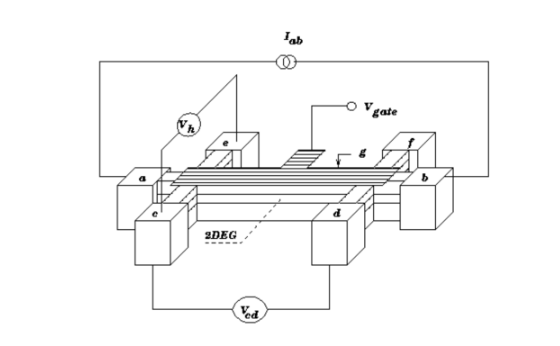
\includegraphics[width=\columnwidth]{figures/fig00_Hallbar_schematic(1).png}
\caption{Illustrative four-terminal Hall-bar contact arrangement consistent with the laboratory contact labels: $a,b$ are current contacts, $c,d,e,f$ are potential contacts and $g$ is the gate. Not to scale; the actual voltage lead pairing and geometric factors must be confirmed with the laboratory wiring.}
\label{fig:contacts}
\end{figure}
\begin{figure}[t]
\centering
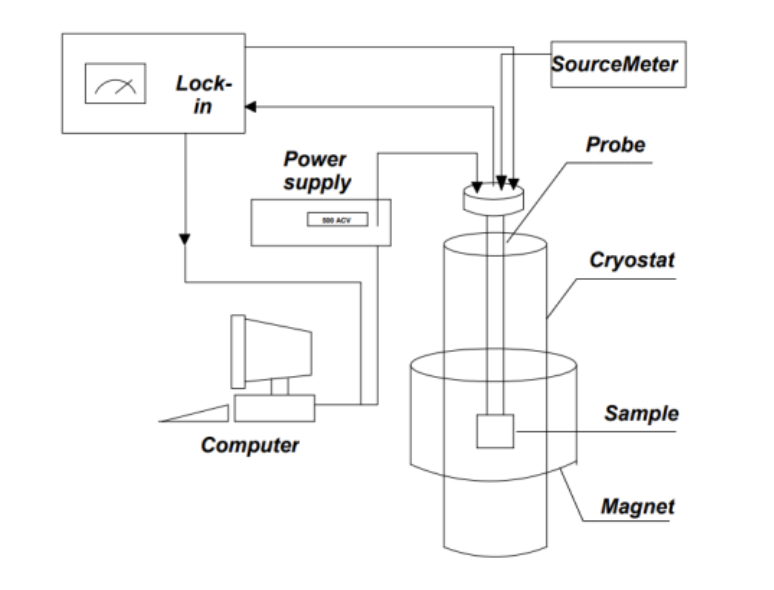
\includegraphics[width=\columnwidth]{figures/fig00_apparatus_schematic.png}
\caption{Conceptual measurement system: AC excitation, two lock-in measurement channels, a cryogenic sample inside the superconducting magnet, a temperature controller, magnet power supply and a gate-voltage source. Lines represent functional links, not verified electrical wiring.}
\label{fig:setup}
\end{figure}




\section{Results}
\subsection{Temperature-dependent resistance}
At $B\simeq0$ and $V_g=0$, the first resistance channel increased from approximately $155\,\Omega$ at $301\,$K to a maximum $6930\,\Omega$ near $148\,$K, and then decreased to approximately $935\,\Omega$ near $4.2\,$K (Fig.~\ref{fig:cooldown}). The peak-to-room-temperature ratio is approximately $44.7$. The response is non-monotonic; it does not establish a unique microscopic mechanism without an independent temperature-dependent carrier density and a controlled scattering model.

\begin{figure}[t]
\centering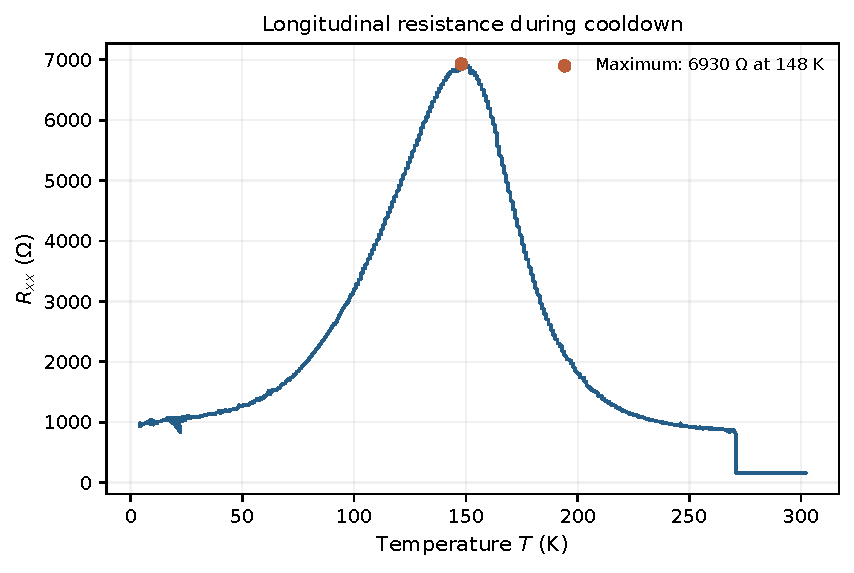
\includegraphics[width=\columnwidth]{figures/fig01_cooldown.pdf}
\caption{Measured longitudinal resistance $R_{xx}$ during cooldown at approximately zero field and zero gate bias. The maximum $6930\,\Omega$ occurs near $148\,$K. The plotted signal has not been corrected for Hall-bar geometry.}
\label{fig:cooldown}
\end{figure}

\begin{figure}[t]
\centering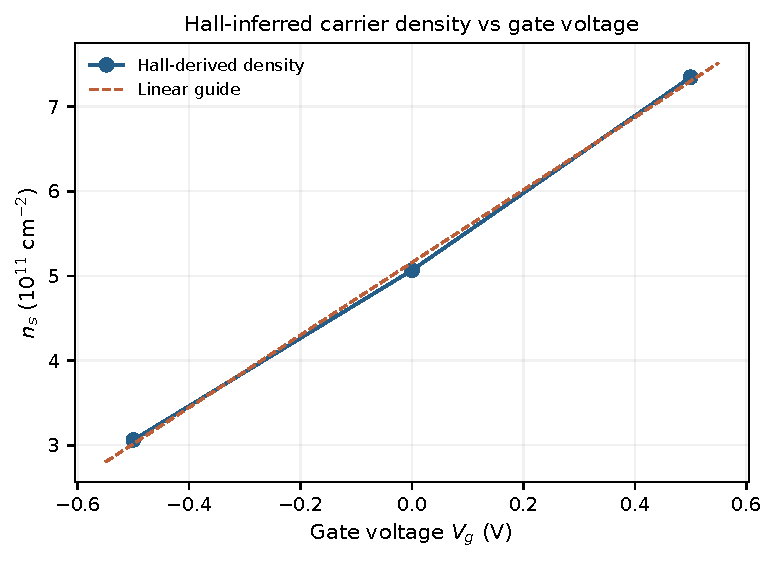
\includegraphics[width=\columnwidth]{figures/fig04_density_vs_gate.pdf}
\caption{Carrier sheet density inferred from the three low-field Hall slopes. The straight dashed line is a linear guide, not a proof of an ideal constant-capacitance gate. Systematic error bars are not available.}\label{fig:gate_density}
\end{figure}

\subsection{Classical Hall response}
At low magnetic field values and zero gate voltage, a linear fit of the Hall resistance against the magnetic field (eq.\ref{eq:hall}) has produced a slope $S_H=1231.9 \pm 3.0 [{\Omega\over T}]$ , from which a charge carrier concentration was extracted, amounting to $n_s= {1\over S_H e}=(5.067\pm 0.012)\times10^{11} [\mathrm{cm}^{-2}]$ (fig.\ref{fig:classHall}).
\begin{figure}[t]
\centering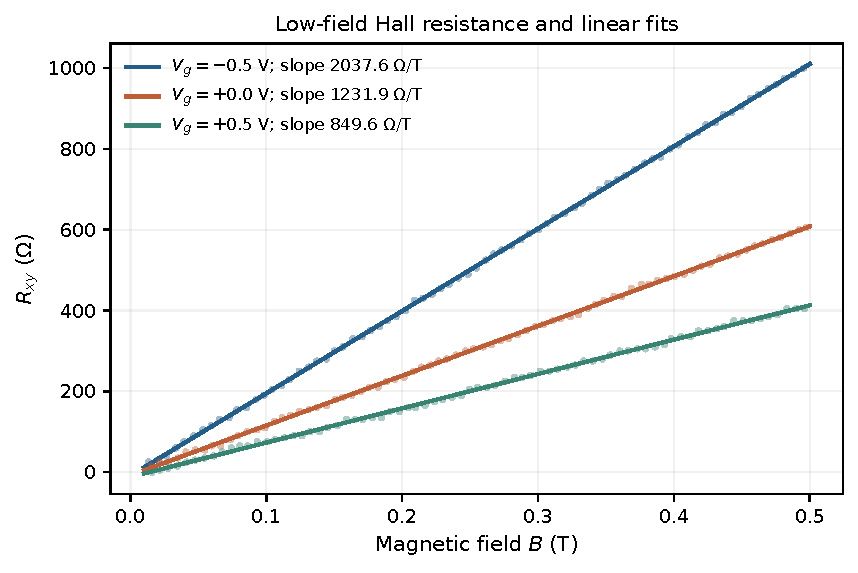
\includegraphics[width=\columnwidth]{figures/fig03_lowfield_fits.pdf}
\caption{Low field Hall resistance for different gate voltages, along with corresponding linear fits for field values $0<B<0.5[T]$.}
\label{fig:classHall}
\end{figure}
\subsection{Comparison with low temperature Hall sweep}
At temperatures $1.7K<T<4.2K$, the hall resistance $R_{xy}$ was measured against the magnetic field for gate bias voltages $V_g=-0.5V,0V,0.5V$. (Fig.~\ref{fig:plateaus}). The resulting plateau values were then extracted and compared to the theoretical expectation of $R_{xy}={h\over\nu e^2}$ for $\nu=1,2,3,\dots$ (fig.\ref{fig:plateau_values}). The best fit was for the visible plateaus corresponding to even values of $\nu$, as would be the case under spin aliasing. The value we got for $R_K$ was $a_1=23.61\pm0.024 [k\Omega]$, which is a significant undershoot of the theoretical value of $R_K={h\over e^2}\approx 25.81[k\Omega]$, with $N_\sigma(R_k,a_1)=92$.
(
an exploratory fit to candidate high field features yields $R_K^{\mathrm{fit}}=(23.61±0.024),\mathrm{k}\Omega$this differs substantially from the theortical value $R_K=25.8128,\mathrm{k}\Omega$. The assignment of integer filling factors,including the possible role of unsolved spin splitting, remains provisional. Consequently the fitted value cannot be regraded as a calibrated determination of the resistance quantum 
)
\begin{figure}
    \centering
    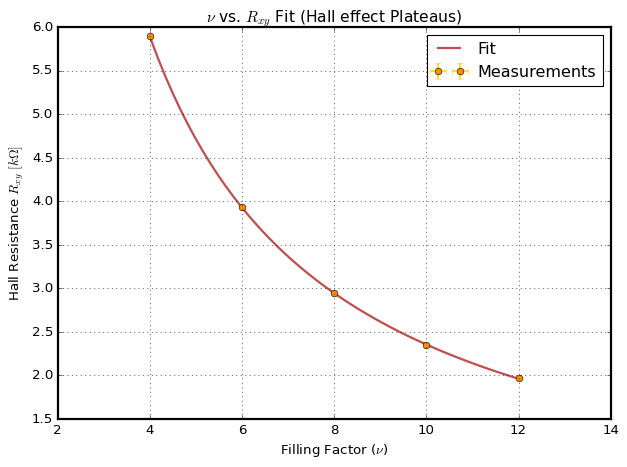
\includegraphics[width=\columnwidth]{Vg_0_hallPlateauValues.png}
    \caption{Inverse first power fit ($a_0+a_1/\nu$) of the measured hall resistance against $\nu$. We obtained $a_0\approx0$ (relative error over $50\%)$ and $a_1=23.61\pm0.024 [k\Omega]$, the expected value being ${h\over e^2}=25.81[k\Omega]$.}
    \label{fig:plateau_values}
\end{figure}



\begin{figure}[t]
\centering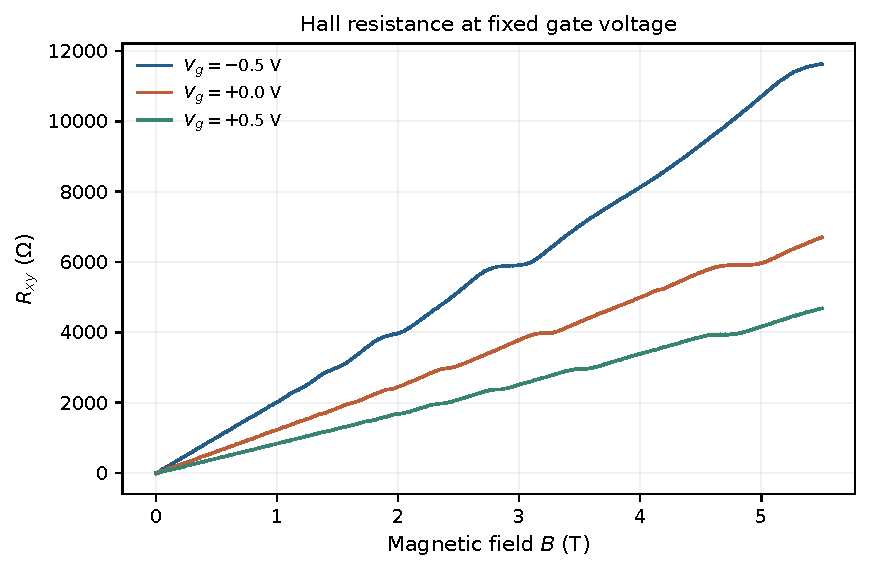
\includegraphics[width=\columnwidth]{figures/fig02_hall_full.pdf}
\caption{Measured Hall resistance $R_{xy}$ at temperatures in the range $1.7K<T<4.2K$ for gate bias voltages $V_g=-0.5V,0V,0.5V$.}
\label{fig:plateaus}
\end{figure}
\begin{figure*}[tbp]
\centering
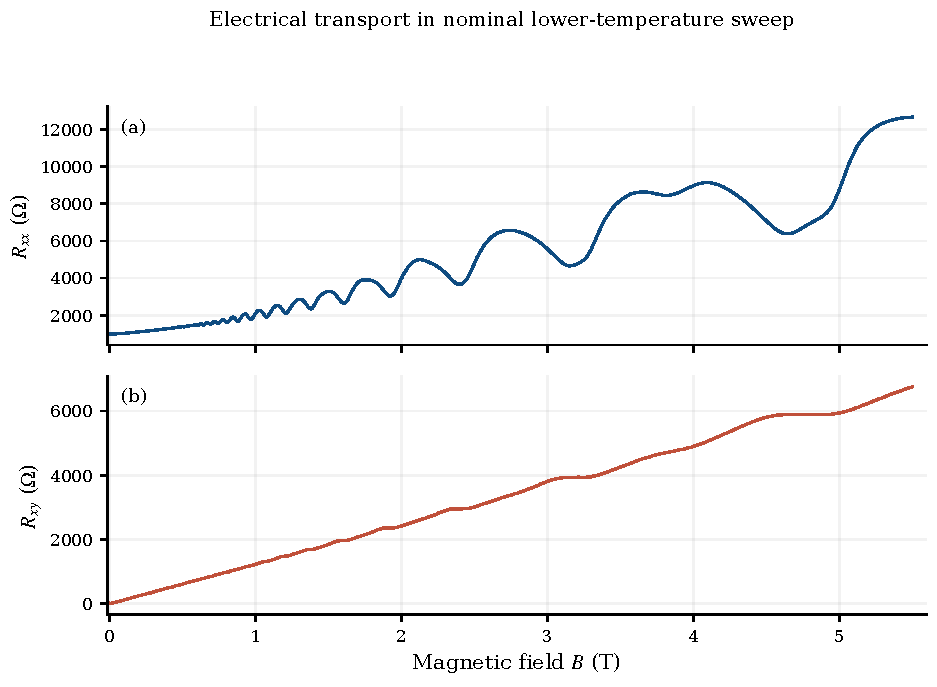
\includegraphics[width=.88\textwidth]{figures/fig16_lowT_measured_vs_auxiliary.pdf}
\caption{The two \emph{primary measured observables} during the nominal lower-temperature magnetic-field sweep: (a) longitudinal-like resistance $R_{xx}(B)$; (b) Hall-like resistance $R_{xy}(B)$. These transport traces remain present even where the separate auxiliary thermometer channel is unavailable (Fig.~\ref{fig:temperature_drift}). The provisional channel mapping and unknown actual sample temperature limit interpretation.
}
\label{fig:lowT_primary}\end{figure*}

\subsection{Gate-voltage dependence of carrier density}
Figure~\ref{fig:gate_density} shows that the low-field Hall-derived density increases from $3.063\times10^{11}\,\mathrm{cm}^{-2}$ at $V_g=-0.5\,$V to $7.346\times10^{11}\,\mathrm{cm}^{-2}$ at $V_g=+0.5\,$V, a factor of approximately $2.40$. The central finite difference gives
\begin{align}
\frac{\Delta n_s}{\Delta V_g}&\simeq4.28\times10^{11}\ \frac{\mathrm{cm}^{-2}}{\mathrm{V}},\nonumber\\
\frac{C_g}{A}&=(6.86\pm0.05)\times10^{-4}\ \mathrm{F/m^2}.
\end{align}


Figure~\ref{fig:fixed_field_gate} displays gate sweeps at six nominal fixed fields between approximately $0$ and $5.5\,$T. At many magnetic fields, increasingly negative gate bias produces larger resistance, consistent with carrier depletion. The variations are not strictly monotonic across all traces: magnetotransport structure and the approach to the resistance measurement ceiling complicate direct interpretation. Notably, repeated exact readings of $25565\,\Omega$ raise concern about instrument range clipping or readout limits; the original instrument configuration is required to confirm that diagnosis. Such readings must not be used as ordinary uncensored values in nonlinear fits.
\begin{figure}[tbp]
\centering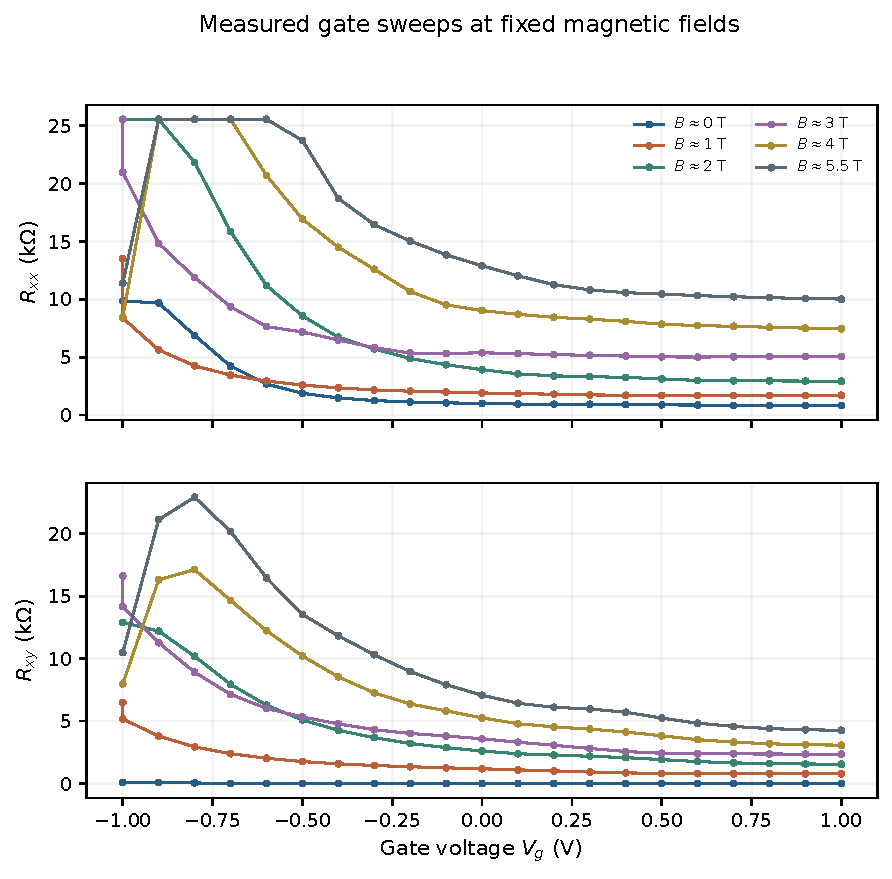
\includegraphics[width=.88\columnwidth]{figures/fig06_fixed_field_gate.pdf}
\caption{Measured $R_{xx}(V_g)$ and $R_{xy}(V_g)$ at nominal fixed fields $B\simeq0,1,2,3,4,5.5\,$T. Values equal to $25565\,\Omega$ may be clipped and require validation before fitting.}\label{fig:fixed_field_gate}
\end{figure}

A useful direct comparison is possible at $B\simeq0$, where the separately recorded \texttt{t\_0.txt} and \texttt{b0.txt} files contain valid thermometer values near $4.15\,$K and $1.71\,$K, respectively. Figure~\ref{fig:gatepair} displays their raw gate-dependent $R_{xx}$ traces. At zero gate bias the instrument readings are approximately $1000$ and $900\,\Omega$ in the two files, respectively. Both curves increase sharply under large negative bias, consistent with depletion, but this alone does not prove a critical transition. For the other \texttt{b1}--\texttt{b5} fixed-field files, the recorded temperature is zero or unavailable and no accurate low-temperature labels are assigned.
\begin{figure}[tbp]
\centering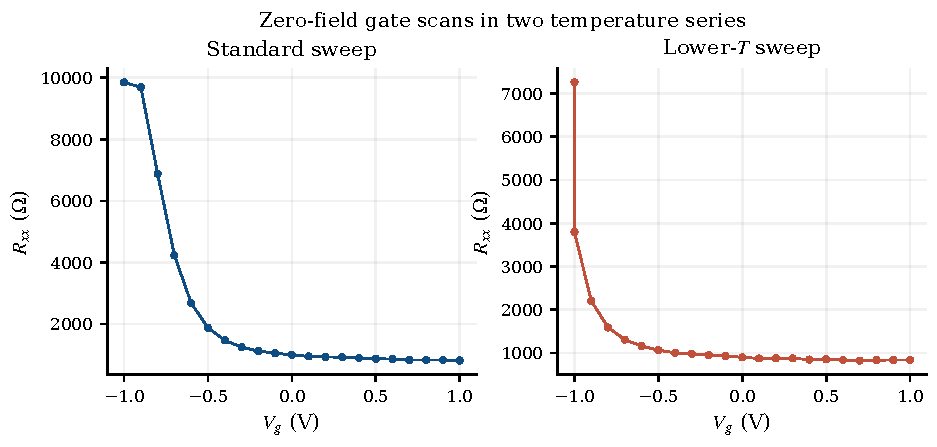
\includegraphics[width=\columnwidth]{figures/fig14_gate_lowfield_comparison.pdf}
\caption{Raw zero-field $R_{xx}(V_g)$ curves from two independently logged gate sweeps with valid temperatures near $4.15$ and $1.71\,$K. Voltage sweeps contain duplicate endpoint records, all retained in the plot.}
\label{fig:gatepair}
\end{figure}

\subsection{Fermi energy estimated from Hall density}
From the inferred carrier sheet densities for different gate voltages (Fig.\ref{fig:gate_density}) we calculated the Fermi energy (eq.\ref{eq:fermi}) associated with each (Table.\ref{tab:fermi}).

\begin{table} [h]
\caption{Fermi energy values inferred from the carrier density figures obtained from the low field hall slopes for different gate bias voltages.}
\begin{ruledtabular}
\begin{tabular}{ccc}
$V_g$(V)&$n_s$ \ ($10^{11}\,\mathrm{ cm}^{-2}]$&$E_F-E_0$ \ (meV)\\\hline

$-0.5$ & $3.0632 \pm 0.0045$ & $10.945\pm 0.016$\\
$0$ & $5.0667 \pm 0.0122$ & $18.103\pm 0.044$\\
$+0.5$ & $7.3462\pm 0.0302$ & $26.248 \pm 0.108$
\\\end{tabular}
\end{ruledtabular}
\label{tab:fermi}
\end{table}

\subsection{Effective electrostatic gate separation}
For a representative dielectric constant $\epsilon_r=12.7$, the ideal capacitor equivalent distance is $d_{\mathrm{eff}}=(163.9\pm1.2)\,$nm. This distance is \emph{not} a direct measure of the physical 2DEG thickness or a uniquely determined heterostructure depth. The change in density from $-0.5$ to $0\,$V is $2.00\times10^{11}\,\mathrm{cm^{-2}}$, whereas the change from $0$ to $+0.5\,$V is $2.28\times10^{11}\,\mathrm{cm^{-2}}$. Thus the three points should not be overinterpreted as establishing exact linearity.

\subsection{Magneto-transport at zero gate voltage}
Figure~\ref{fig:magnetotransport} compares the two zero-gate field sweeps. $R_{xx}$ exhibits substantial nonmonotonic field dependence, while $R_{xy}$ initially grows nearly linearly, as expected for a Hall-like channel. This field dependence is not reproduced by the simplest one-band constant-scattering-time Drude model. The traces do not, by themselves, establish either SdH oscillations or quantized Hall plateaus. In particular, peaks in raw magnetoresistance should not be assigned to individual Landau levels without a reproducible $1/B$ analysis and a consistent longitudinal/transverse contact calibration.
\begin{figure}[tbp]
\centering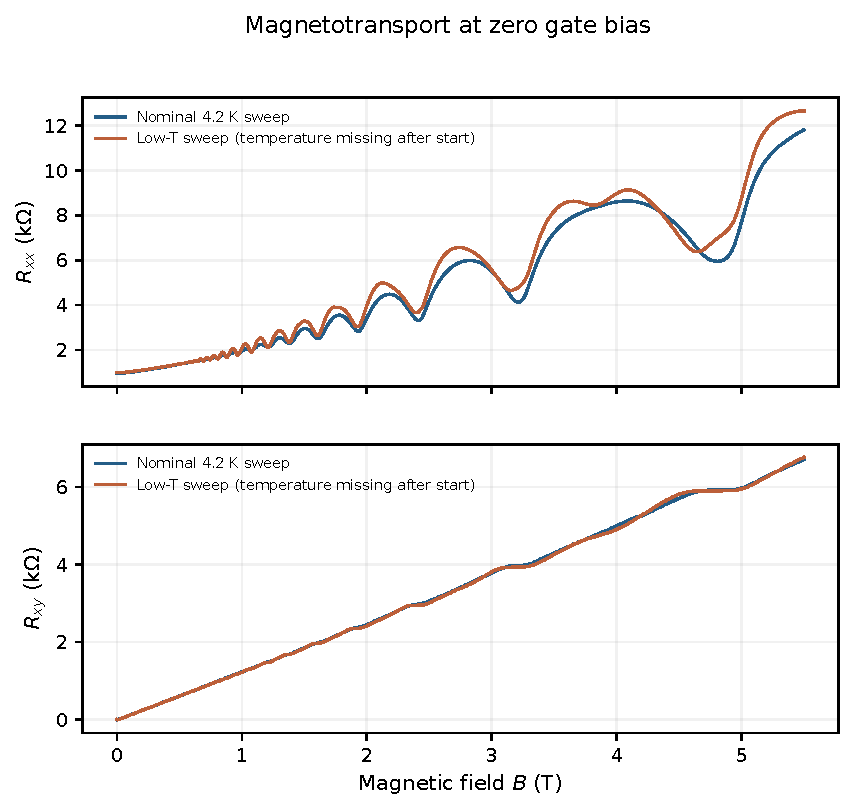
\includegraphics[width=.88\columnwidth]{figures/fig05_magnetotransport.pdf}
\caption{Two supplied zero-gate field sweeps displaying $R_{xx}(B)$ and $R_{xy}(B)$. Thermometer data for the nominally colder sweep are invalid over much of the run. The curves are measured instrument resistances, not geometry-corrected sheet resistivities.}\label{fig:magnetotransport}
\end{figure}
Additional field sweeps at fixed gate voltages reveal a strong dependence on $V_g$ (Fig.~\ref{fig:gate_field}). Their variation is qualitatively consistent with the substantial gate dependence of carrier density inferred from the low-field Hall coefficients. Quantitative comparisons in the high-field regime are limited by temperature drift and channel-mixing uncertainties.
\begin{figure}[tbp]
\centering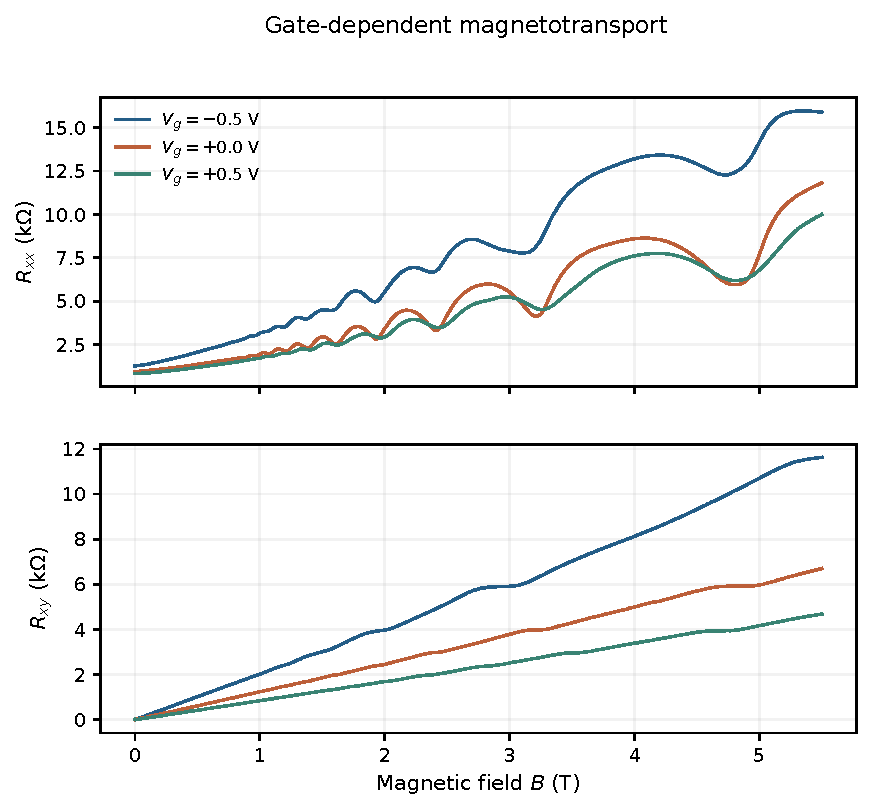
\includegraphics[width=.88\columnwidth]{figures/fig09_gate_dependent_field.pdf}
\caption{Measured $R_{xx}(B)$ and $R_{xy}(B)$ at fixed gate voltages $-0.5,0,+0.5\,$V. Strong field- and gate-dependence are apparent. Physical interpretation requires independent verification of contact wiring and temperature history.}\label{fig:gate_field}
\end{figure}

To test the defining complementarity of the IQHE, Fig.~\ref{fig:joint} displays the simultaneously acquired $R_{xy}(B)$ and $R_{xx}(B)$ from the standard zero-gate sweep. The upper panel is normalized by the quantum resistance $R_K=h/e^2\simeq25\,812.807\,\Omega$; crosses show theoretical integer-filling predictions $\big(B_\nu,1/\nu\big)$ derived from the low-field Hall density. The lower panel retains the measured longitudinal resistance in ohms. No common interval can be established in this uncorrected dataset where the Hall-like channel is demonstrably flat at a calibrated quantized value \emph{and} the longitudinal-like signal approaches zero. As one concrete example, at $B\simeq4.998\,$T the records give $R_{xx}=7655\,\Omega$ and $R_{xy}=5970\,\Omega$, or $|R_{xy}|/R_K\simeq0.2313$. Nearness to $1/4=0.25$ is not by itself evidence for a $\nu=4$ plateau. Moreover, these are \emph{raw} channel readings, and the contact mapping may need calibration.
\begin{figure}[tbp]
\centering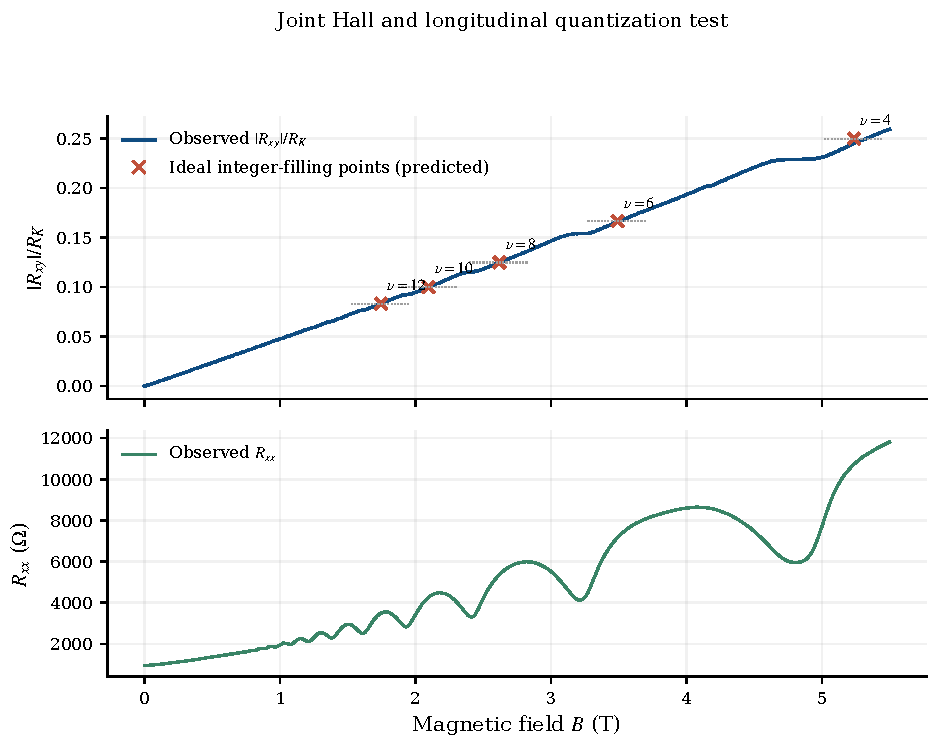
\includegraphics[width=\columnwidth]{figures/fig17_joint_hall_longitudinal.pdf}
\caption{Joint test of integer quantum Hall behavior from the supplied standard zero-gate sweep: (a) measured $|R_{xy}|/R_K$ against $B$ with theoretical integer-filling points \emph{(crosses; not experimental plateaus)}; (b) simultaneously measured $R_{xx}$ in ohms. A convincing IQHE plateau would require a stable quantized Hall response and the corresponding longitudinal minimum under validated contact geometry and calibration.}
\label{fig:joint}
\end{figure}
A second diagnostic is the \emph{raw resistance ratio} $|R_{xy}|/R_{xx}$, plotted in Fig.~\ref{fig:ratio}. At $B\simeq0.998\,$T it is approximately $0.634$, at $B\simeq1.999\,$T approximately $0.718$, and at $B\simeq4.998\,$T approximately $0.780$. Its dependence on the field is not the linear $\mu B\,W/L$ predicted by a constant-$\tau$ one-carrier Drude approximation. However, the quotient is \emph{not} $|\rho_{xy}|/\rho_{xx}$ without geometry correction, and cannot independently establish an IQHE state or an absolute mobility. In particular, the conductivity tensor in Eq.~\eqref{eq:conductivity} cannot be reconstructed reliably from these two instrument outputs without the sample geometry and a verified contact assignment.
\begin{figure}[tbp]
\centering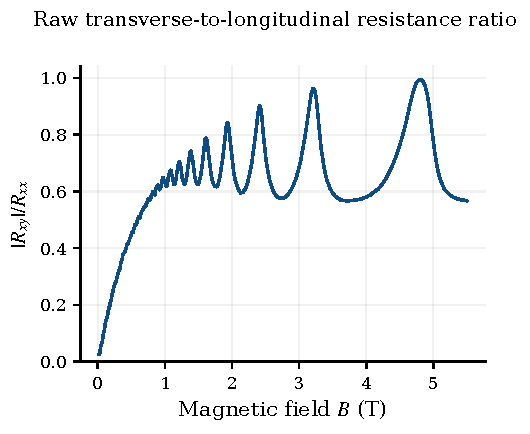
\includegraphics[width=\columnwidth]{figures/fig18_ratio_raw.pdf}
\caption{Descriptive ratio of the two simultaneous instrument resistances, $|R_{xy}|/R_{xx}$, during the standard zero-gate magnetic-field sweep. It must not be confused with the Hall angle $|\rho_{xy}|/\rho_{xx}$ or used to infer mobility without the contact geometry.}
\label{fig:ratio}
\end{figure}
Assuming a single occupied subband, twofold spin degeneracy at zero field, and $m^*=0.067m_e$, Eq.~\eqref{eq:fermi} gives $E_F-E_0=(18.1\pm0.04)\,$meV at $V_g=0$ (Hall fit error only, holding $m^*=0.067m_e$ fixed).

\subsection{Expected integer filling-factor fields}
The Hall-derived carrier density also yields the theoretical field scale $n_sh/e\simeq20.95\,$T. Predicted integer filling fields and the ideal quantized resistance levels are listed in Table~\ref{tab:fill}. They are \emph{not} identified plateaus in the supplied data.
\begin{table}[tbp]
\caption{Model predictions from the zero-gate Hall density, not identified experimental Hall plateaus.}\label{tab:fill}
\begin{ruledtabular}
\begin{tabular}{ccc}
$\nu$&$B_\nu$ (T)&$h/(\nu e^2)$ ($\Omega$)\\\hline
12&1.746&2151.1\\
10&2.095&2581.3\\
8&2.619&3226.6\\
6&3.492&4302.1\\
4&5.239&6453.2
\end{tabular}
\end{ruledtabular}
\end{table}

\begin{figure}[tbp]
\centering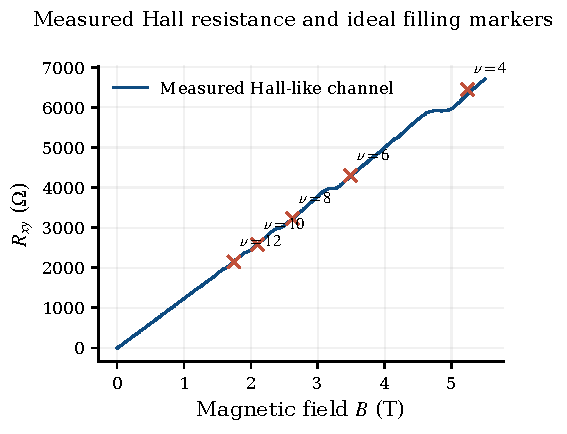
\includegraphics[width=\columnwidth]{figures/fig15_IQHE_benchmark.pdf}
\caption{Hall-channel measurements (solid line) and ideal integer-filling benchmarks (crosses) computed from the zero-gate Hall density. Crosses denote isolated theoretical pairs $(B_\nu,h/\nu e^2)$, \emph{not} measured plateaus.}
\label{fig:iqhebenchmark}
\end{figure}

Figure~\ref{fig:iqhebenchmark} compares the measured Hall-like channel with the five nominal integer-filling point predictions from Table~\ref{tab:fill}. A near coincidence of an individual point with $h/(\nu e^2)$ does not establish a plateau: a field interval with a sufficiently flat Hall response \emph{and} a correlated longitudinal minimum is required. The raw high-field longitudinal signal remains substantial, and the contact geometry is not independently established. We therefore report these as reference benchmarks only. The original example report also contains a grader's warning about the geometry needed for an appropriate Hall resistivity interpretation; a factor from that particular sample cannot safely be applied to an unknown wiring configuration.

\subsection{SdH periodicity}
For $V_g=0$ and temperatures $1.7K < T < 4.2K$, the longtitudinal resistance $R_{xx}$ was measured against $1/B$ (Fig.\ref{fig:SdH_peaks}). It exhibited oscillations with a period of $\Delta(1/B)=0.0988\pm 0.0053\ [T^{-1}]$, which is consistent with the period derived from the charge carrier density, $\Delta(1/B)=0.095459\pm 0.000094\ [T^{-1}]$.

Furthermore, the oscillation amplitude was measured as a function of the field $B$ and modeled according to the following fit function (Fig.\ref{fig:SdH_fit}): \begin{equation} y=a_0e^{-a_1\over x} \end{equation}  This form represents the limit ${X \over \mathrm{sin}(X)}\approx1$ for eq.\ref{eq:sdh}, which is relevant for fields $1<B<5\ [T]$. (The SdH amplitude is modeled by \begin{equation} A(B,T)=A_0\frac{X}{\sinh X} \exp\left(-\frac{B_D}{B}\right), \end{equation} where \begin{equation} X=\frac{2\pi^2 k_B Tm^*}{\hbar eB}, \qquad B_D=\frac{\pi m^*}{e\tau_q}.\end{equation} The thermal damping factor cannot be neglected throughout the investigated field interval.)
\begin{figure}
    \centering
    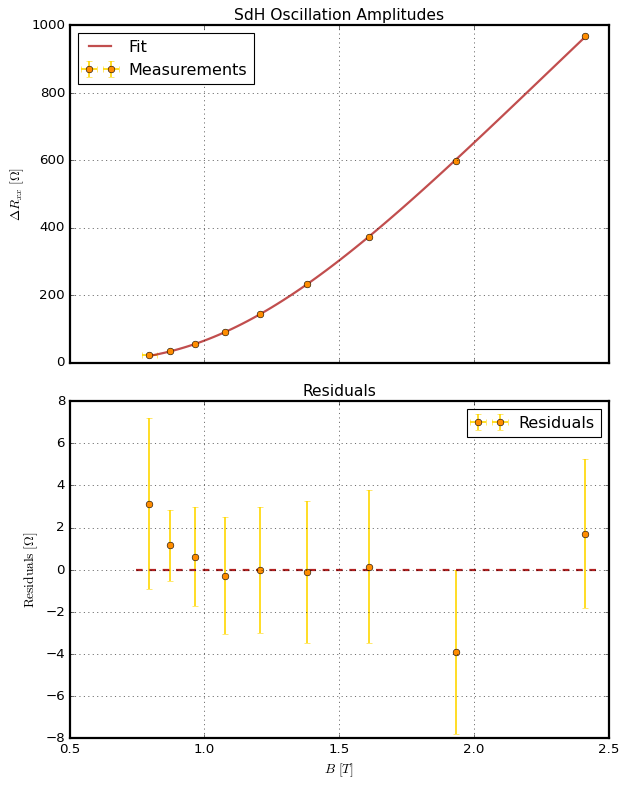
\includegraphics[width=1\linewidth]{SdH_amplitudes_residuals.png}
    \caption{Shubnikov de-Haas oscilation amplitudes for $V_g=0$ and $T\approx4\ [K]$, modeled as an exponential of $a_1B^{-1}$. the fit yields $a_1=4.599\pm0.014\ [T]$ with $p_{val}=0.93$, $\chi^2_{red}=0.34$.}
    \label{fig:SdH_fit}
\end{figure}

From eq.\ref{eq:sdh} one expects $a_1={\pi m* \over e\tau_q}$, so we extracted a Dingle time $\tau_q=0.2602\pm0.008\ [p\mathrm {Sec}]$ and a corresponding Dingle mobility $\mu_q=6831\pm21\ [{\mathrm{cm}^2\over\mathrm{V\times Sec}}]$.


\begin{figure}
    \centering
    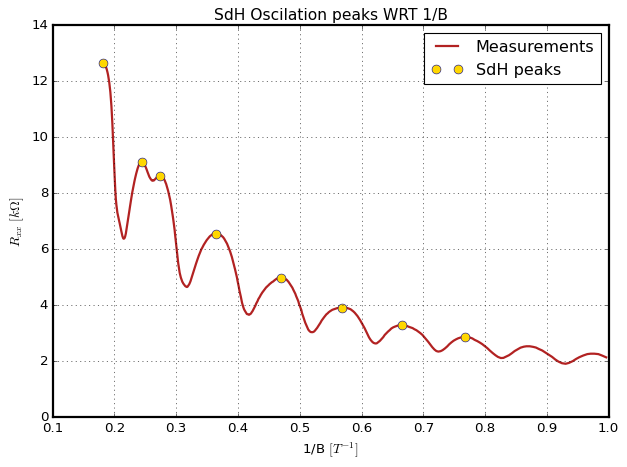
\includegraphics[width=1\linewidth]{SdH_peaks.png}
    \caption{Shubnikov de-Haas oscilation maxima for $V_g=0$. in all but one of the periods, the peaks are resolveble only to pairs of $\nu$ integer values.}
    \label{fig:SdH_peaks}
\end{figure}
The experimental instructions request a table of microscopic transport parameters at nominal $4.2$ and $1.7\,$K. Table~\ref{tab:micro} separates directly supported quantities, conditional model-derived estimates, and unidentifiable parameters. At zero gate, using the near-zero-field resistance $R_{xx}\simeq955\,\Omega$ and the Hall density, the standard Drude analysis would give
\begin{equation}
\mu=\frac{L/W}{n_seR_{xx}}\simeq (L/W)\,1.29\times10^4\ \mathrm{cm^2/(V\,s)},
\end{equation}
\begin{equation}
\tau_{\mathrm{tr}}=\frac{m^*\mu}{e}\simeq(L/W)\,0.491\ \mathrm{ps}.
\end{equation}
The unknown geometric ratio $L/W$ is \emph{not} assumed to be one. These are scaling relations, not measured mobility or lifetime. The quantum lifetime $\tau_q$ additionally requires a physically validated SdH amplitude analysis with a reliable temperature record, so it is unassigned. The same caution applies to the other nominally lower-temperature sweep.
\subsection{Gate leakage current}
In selected fixed-field sweeps, the magnitude of the recorded leakage current increases sharply at positive gate voltages (Fig.~\ref{fig:gate_leakage}). Currents of order $10^{-10}$--$10^{-9}\,$A occur across substantial bias ranges, while some data reach order $10^{-7}\,$A close to $+1\,$V. This change suggests that the largest positive biases should not be interpreted through a purely capacitive model without an explicit leakage assessment. The density-vs-gate estimates above use the field sweeps at $V_g\in\{-0.5,0,0.5\}\,$V; the leakage behavior of the separate fixed-field scans does not automatically establish equal leakage in those datasets.
\begin{figure}[tbp]
\centering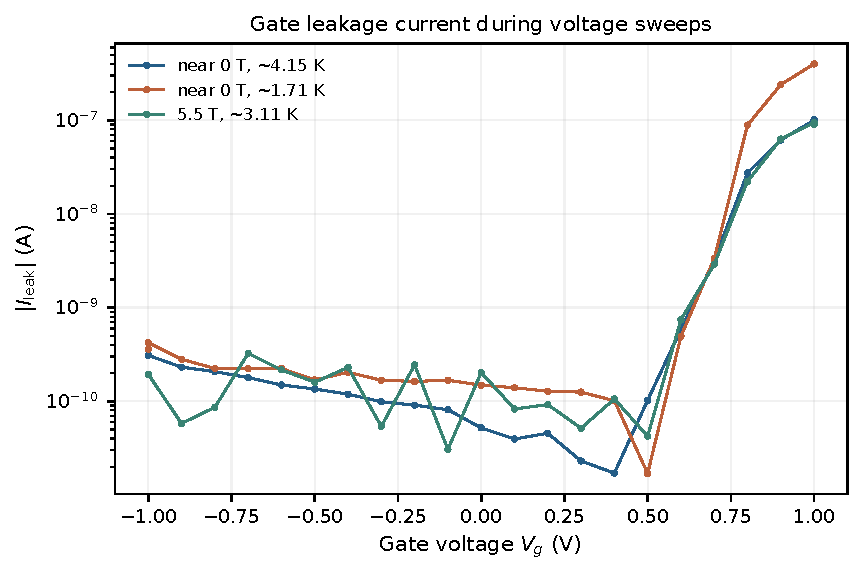
\includegraphics[width=\columnwidth]{figures/fig07_gate_leakage.pdf}
\caption{Absolute leakage current recorded during representative gate sweeps at different fixed fields. The logarithmic ordinate displays both small baseline values and the sharp rise at large positive gate bias.}\label{fig:gate_leakage}
\end{figure}
\begin{table*}[tbp]
\caption{Zero-gate transport parameter status. Numerical entries are conditional on the provisional Hall-channel identification and simple single-subband model. ``Not determined'' indicates missing metrological inputs, not a zero value.}
\label{tab:micro}
\begin{ruledtabular}
\begin{tabular}{lll}
Parameter & \shortstack{Standard sweep\\(starts near $4.2$ K)} & \shortstack{Nominal lower-$T$ sweep\\(thermometer mostly missing)}\\\hline
Hall density, $n_s$ & $5.067\times10^{11}$ cm$^{-2}$ & $\sim5.05\times10^{11}$ cm$^{-2}$\\
Fermi energy $E_F-E_0$ (model-derived) & $18.1$ meV & $\sim18.1$ meV\\
Mobility $\mu$ & $(L/W)\times1.29\times10^4$ cm$^2$/(V s) & Not determined (geometry, conditions)\\
Transport lifetime $\tau_{\mathrm{tr}}$ & $(L/W)\times0.491$ ps & Not determined\\
Quantum/Dingle lifetime $\tau_q$ & Not determined & Not determined\\
Candidate inverse-field period & $0.10296$ T$^{-1}$ & $0.10260$ T$^{-1}$
\end{tabular}
\end{ruledtabular}
\end{table*}
\subsection{Data quality and limitations}
In the lower temperature magnetic field sweep, out of $847$ recorded rows, $31$ contain nonzero thermometer readings, initially $1.735\,$K and declining to $1.015\,$K. The first zero reading is recorded at $t=62.225\,$s and $B=0.1977\,$T; the remaining $816$ entries (approximately $96.3\%$ of the scan) are zero. All $816$ are treated as \emph{missing or invalid thermometer readings}. We do not infer that the specimen reached $0\,$K or that its actual temperature followed any particular continuation after loss of readout. The listed equipment specification covers approximately $1.7$--$300\,$K, so even the nonzero entries below $1.7\,$K require a validated sensor and conversion curve before being interpreted quantitatively.

The available $R_{xx}(B)$ and $R_{xy}(B)$ traces remain useful for field-dependent observations, Hall-slope estimates, and exploratory extremum positions. However, accurate thermal damping, inter-sweep amplitude comparisons, and Dingle-lifetime determination require verified sample temperature as a function of field. Consequently, the term \emph{nominal lower-temperature sweep} is used throughout, rather than labeling its full trace as an isothermal $1.7\,$K dataset.

The thermometer output in the standard zero-gate field sweep declines from approximately $4.145\,$K to $3.113\,$K as $B$ approaches $5.5\,$T; the corresponding trace is shown in Fig.~\ref{fig:temperature_drift}. The nominally lower-temperature magnetic-field sweep begins with a recorded $1.735\,$K and has only $31$ nonzero temperature readings out of $847$ rows; from $B=0.1977\,$T onward, the remaining $816$ zero entries are flagged as invalid readout, not absolute zero. As shown in Fig.~\ref{fig:lowT_primary}, the physical measurement targets $R_{xx}(B)$ and $R_{xy}(B)$ remain recorded throughout. The field-dependent data therefore cannot be considered strictly isothermal, and a quantitative SdH amplitude comparison between two fixed temperatures is not justified.

\begin{figure}[tbp]
\centering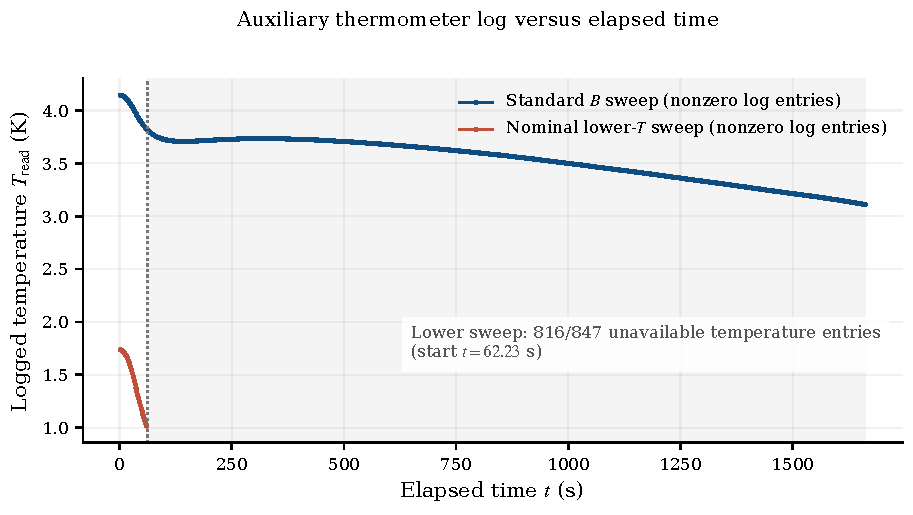
\includegraphics[width=\columnwidth]{figures/fig08_temperature_drift.pdf}
\caption{\emph{Auxiliary thermometer diagnostic} $T_{\mathrm{read}}(t)$ versus elapsed time for the two zero-gate magnetic-field sweeps. Invalid zero readouts in the nominal lower-temperature file are omitted, and the shaded interval (from $t=62.225\,$s onward) shows the missing portion of that readout. The main experimental responses are $R_{xx}(B)$ and $R_{xy}(B)$, not a thermometer response to field.}\label{fig:temperature_drift}
\end{figure}

The exact repeated readings of $25565\,\Omega$ in selected gate scans may indicate a readout ceiling; no correction for such clipping has been applied. The missing thermometer readings cannot be assigned a physical value, and lead pairing, geometry, instrument gain, and model choice remain sources of unquantified systematic uncertainty.

\section{Discussion}
\label{sec:discussion}

\subsection{Electrostatic control of the electron density}

The low-field Hall response is nearly linear for $B<0.5\,\mathrm{T}$. At zero gate bias, the fitted slope $S_H=(1231.9\pm3.0)\, \Omega\,\mathrm{T}^{-1}$ implies a carrier sheet density of $n_s=(5.067\pm0.012)\times10^{11}\,\mathrm{cm}^{-2}$ within the single-carrier approximation.
The density increases with positive gate bias, consistent with electrostatic accumulation. The endpoint-derived gate capacitance per unit area is $(6.86\pm0.05)\times10^{-4} \,\mathrm{F\,m^{-2}}$. For $\epsilon_r=12.7$, the corresponding idealized electrical separation is $(163.9\pm1.2)\,\mathrm{nm}$. These uncertainties are statistical only and exclude possible errors in contact assignment, field calibration, dielectric properties, and parallel conduction \cite{ando1982,weisbuch1991}. We do not interpret $d_{\rm eff}$ as a measured quantum-well thickness. \subsection{Temperature-dependent transport} The cooldown trace has a maximum near $148\,$K, falling at both higher and lower temperature. The empirical $10$--$120\,$K power law $p=3.25\pm0.02$ and the $160$--$250\,$K activation scale $E_a=79.5\pm1.0\,$meV carry \emph{formal fit errors only}. The unusually small statistical errors do not distinguish phonon scattering from changes in occupied conducting channels, carrier freeze-out, or parallel conduction; a temperature-dependent Hall density would be necessary. Different microscopic contributions to a GaAs-based two-dimensional system are documented in reviews of semiconductor 2DEGs\cite{ando1982,weisbuch1991}. The fit windows were chosen for numerical description, not to establish a unique activated or Bloch--Gr\"uneisen regime.

\subsection{High-field magneto-transport}
The defining test of integer quantum Hall transport is not merely that the Hall-like resistance crosses a theoretical value, but that a finite-field Hall plateau is observed \emph{together} with suppression of longitudinal dissipation. The corresponding conductivity requires both geometry-corrected resistivity components [Eq.~\eqref{eq:conductivity}]\cite{klitzing1980,halperin1982,buttiker1988}. In our archive the raw $R_{xx}$ channel remains appreciable near nominal integer-filling markers and the mapping of contacts is not independently known. Accordingly, the reported $|R_{xy}|/R_K$ plot and the resistance ratio $|R_{xy}|/R_{xx}$ are diagnostic comparisons, \emph{not a verification} of quantized Hall conductivity. No sample-specific factor from the comparison student paper is applied to the present records.

A detrended longitudinal-channel analysis yields a repeatable candidate period near $0.103\,$T$^{-1}$ at zero gate voltage, compared with $0.09545\,$T$^{-1}$ predicted from the Hall-inferred density. More importantly, the candidate period varies by only about $1.2\%$ across the $-0.5$ to $+0.5\,$V gate range, whereas the one-subband prediction changes substantially. Small extrema-index regression errors therefore cannot validate the proposed SdH identification: uncertainties in background subtraction, peak selection, contact mixing, parallel conducting channels, or an instrumental field-correlated signal remain plausible. Coleridge's analysis of quantum versus transport scattering emphasizes that even a genuine oscillatory signal requires a separately justified lifetime interpretation\cite{coleridge1991,dingle1952,shoenberg1984}. We make no independent SdH-density, spin-splitting, or Dingle-lifetime claim.

\subsection{Transport and quantum scattering lifetimes}
The transport mobility and lifetime cannot be reported as absolute measured values while the geometric ratio $L/W$ and the voltage-channel assignment are not verified. The conditional scalings in Table~\ref{tab:micro} show how these values would depend on a subsequently verified sample geometry. The quantum (Dingle) lifetime requires a validated SdH amplitude envelope and reliable temperature history: the observed candidate period has not passed an independent gate-dependence test, and the temperature record is incomplete. In particular, formal fit errors on the putative minima indices are not substitutes for uncertainty in the identification of the physical oscillations\cite{coleridge1991,dingle1952,shoenberg1984}. The correct response is to state that $\tau_q$ and absolute $\tau_{\mathrm{tr}}$ remain undetermined, rather than assigning values by treating raw instrument resistances as calibrated sheet resistivity.

\subsection{Experimental limitations}
At several fixed magnetic fields the resistance increases as gate bias becomes more negative, but clipping-like repeated $25565\,\Omega$ readings and elevated positive-bias leakage hinder quantitative model fits. Electrostatic depletion is compatible with the trend, whereas a metal--insulator transition cannot be established from one temperature series without scaling tests\cite{lee1985,ando1982}. The nominal lower-temperature magnetic-field sweep contains 816 zero-valued thermometer entries out of 847 readings, beginning at $B=0.1977\,$T. Since the electrical channels continue, these are missing readouts, \emph{not} $0\,$K sample temperatures or evidence that a temperature sweep was performed. A known $T(B)$ is nevertheless required for the thermal SdH attenuation factor. We therefore omit an unreliable extraction of $\tau_q$, and report mobility and $\tau_{\rm tr}$ only as $L/W$-dependent scalings until the sample geometry and electronics are documented.

\emph{All analyzed data came from an archived dataset provided after a failed experimental session, not from a successful run performed by the authors. Before submission, the reproducibility package must be made public on GitHub subject to laboratory permission, and the placeholder URL in Sec.~III must be replaced. The most valuable additional measurements are a verified Hall-bar pinout and probe spacing, recorded AC current and phase settings, stable thermometer logging across both nominal cryogenic temperatures, field sweeps in both polarities to isolate odd Hall response, and repeated magnetic-field traces with sufficient precision to establish or reject the observed inverse-field pattern. These controls would enable an uncertainty-aware comparison of $n_s^{\rm Hall}$ and $n_s^{\rm SdH}$ and potentially a calibrated quantum Hall conductivity.
}

\begin{acknowledgments}

The authors thank the Lab-C faculty for supplying the experimental equipment and coordinating the schedule of the measurements, instructor Nir Levin for his guidance and enabling us to work in spite of the prevailing conditions of the experimental system, and finally we thank the anonymous providers of the experimental data for this analysis, without whom it couldn't be performed at all.

\end{acknowledgments}

% References

\begin{thebibliography}{15}


\bibitem{weisbuch1991} C. Weisbuch and B. Vinter, \textit{Quantum Semiconductor Structures: Fundamentals and Applications} (Academic Press, 1991).
\bibitem{ando1982} T. Ando, A. B. Fowler, and F. Stern, Rev. Mod. Phys. \textbf{54}, 437 (1982).

\bibitem{ashcroft1976} N. W. Ashcroft and N. D. Mermin, \textit{Solid State Physics} (Holt, Rinehart and Winston, 1976).
\bibitem{datta1995} S. Datta, \textit{Electronic Transport in Mesoscopic Systems} (Cambridge University Press, 1995).

\bibitem{halperin1982} B. I. Halperin, Phys. Rev. B \textbf{25}, 2185 (1982).
\bibitem{buttiker1988} M. B\"uttiker, Phys. Rev. B \textbf{38}, 9375 (1988).
\bibitem{tsui1982} D. C. Tsui, H. L. St\"ormer, and A. C. Gossard, Phys. Rev. Lett. \textbf{48}, 1559 (1982).
\bibitem{chakraborty1995} T. Chakraborty and P. Pietil\"ainen, \textit{The Quantum Hall Effects: Integral and Fractional} (Springer, 1995).
\bibitem{shoenberg1984} D. Shoenberg, \textit{Magnetic Oscillations in Metals} (Cambridge University Press, 1984).
\bibitem{dingle1952} R. B. Dingle, Proc. R. Soc. London A \textbf{211}, 500 (1952).
\bibitem{coleridge1991} P. T. Coleridge, Phys. Rev. B \textbf{44}, 3793 (1991).
\bibitem{lee1985} P. A. Lee and T. V. Ramakrishnan, Rev. Mod. Phys. \textbf{57}, 287 (1985).

\end{thebibliography}
\end{document}

